\documentclass[9pt,twocolumn,twoside]{osajnl}


%\usepackage{csquotes}
\usepackage{tikz}
%\usepackage{graphicx}


\journal{josaa} % Choose journal (ao, josaa, josab, ol)

\setboolean{shortarticle}{false} % true = letter, false = research article

\title{Optical metric in the non-impedance-matched media}

\author[1]{S. A. Mousavi}
\author[2*]{R. Roknizadeh}
\author[3,4]{SH. Dehdashti}
\author[5]{S. Sahebdivan}

\affil[1]{Department of Physics, Faculty of Science, University of Isfahan, Hezar Jerib, Isfahan, 81746-73441, Iran}
\affil[2]{ Department of Physics, Quantum Optics Group, Faculty of Science, University of Isfahan, Hezar Jerib, 81746-73441 Isfahan, Iran}
\affil[3]{State Key Laboratory of Modern Optical Instrumentations, Zhejiang University, Hangzhou 310027, China}
\affil[4]{The Electromagnetic Academy at Zhejiang University, Zhejiang University, Hangzhou 310027, China}
\affil[5]{Quantum Optics, Quantum Nanophysics and Quantum Information, Faculty of Physics, University of Vienna, Boltzmanngasse 5, 1090 Wien}
\affil[*]{Corresponding author: r.roknizadeh@gmail.com}

\dates{Compiled \today}

\ociscodes{(160.1190)  Anisotropic optical materials,(160.3918) Metamaterials, (260.2110)   Electromagnetic optics }

\doi{\url{http://dx.doi.org/10.1364/ao.XX.XXXXXX}}

\begin{abstract}


In the non-magnetic anisotropic media, the behavior of electromagnetic waves depends on the polarization and the direction of the incident light. 
Accordingly, this is the reason that the artificial impedance-matched medium were suggested to be used alternatively in some particular optical devices like invisibility cloak or super lenses to tame some unwanted wave responses like polarization dependent reflections.
Nevertheless, developing the impedance-matched medium is not free of difficulties. 
In this paper, we are comparing the samples of two impedance-matched and non-impedance-matched (non-magnetic) media regarding their optical response in constructing a well-defined metric. 
Our derivatives show the capacity and limits of using the birefringent media as the transformation media, especially in response to the in-the-plane polarization (TM polarization). 
 We find that, in the similar anisotropic condition, the effective geometry of the impedance-matched medium is the same as the geometry perceived by TM polarization (extraordinary light) in an electrical birefringent medium. 


\end{abstract}

\setboolean{displaycopyright}{true}

\begin{document}
\maketitle
\thispagestyle{fancy}
\ifthenelse{\boolean{shortarticle}}{\abscontent}{}

\section{Introduction}




Theoretically, it was a known fact that there is a subtle relation between the electromagnetic constitutive relation of matter and the light trajectories inside the optical medium.
In the mid-seventies, Plebanski formulated the analogy between the empty curved space-time and the magneto-electric media \cite{plebanski1977separation}. 
 But, just in the recent years \cite{yao2014analogy, leonhardt2006general, thompson2011completely} the complete analysis, in term of transformation optics, reveals the essential conditions and fundamental restrictions for such an analogy in practice. 

The underlying principle of such a geometrical analogy is the conformal invariance of electromagnetic fields which allows a diffeomorphism between an arbitrary curved vacuum (called virtual space-time or electromagnetic space) and the designed medium that serves as the real space-time.  
One of the crucial conditions which allow this analogy is the impedance-matched feature of the medium. 
An impedance-matched material is a magneto-electric medium that satisfies the condition: $\mu=\epsilon$. The term "impedance-match" refers to impedance invariant property of the medium ${\mathbf z}=\sqrt {{\epsilon}/{\mu}}=\sqrt {{\epsilon_0}/{\mu_0}}$ compare to vacuum. 
 An impedance-matched medium resembles some of the electromagnetic responses of the vacuum. 
However, as the impedance-matched anisotropic materials are very rare in nature, applying this analogy had been restricted to some theoretical studying \cite{barcelo2005analogue}. 
Fabrication of artificial materials is yet in its infancy. Therefore, the realization of complex synthetic materials like an impedance-matched medium in the broadband of frequencies is not a trivial task. Apparently, it would be of a great advantage if there were an alternative way to avoid the technically cumbersome fabrication \cite{narimanov2009optical, lee2014elliptic, dehdashti2013analogue, visser2013survey, robertson2012theory, wang2011cylindrical, bai2010controllable} and related expenses. 
From the experimental viewpoint, only recently, the practical interests in the analog system raised.

Mainly, because the growing development of the metamaterial technologies \cite{cai2010optical}, brings the hope that vast range of artificial media with unusual electric and magnetic property can be made in practice \cite{cai2010optical, narimanov2009optical}.
 In the scientific literature, people ease the impedance-matched condition by using anisotropic media with electrical anisotropy, i.e. non-magnetic media, and use of the polarized light. The construction of these media is more practical than the impedance-matched, anisotropic medium. Nevertheless, this approach would restrict the control of light to one single polarization. Therefore, the optical device naturally has not the full functionality. 
However, there is still the lack of comprehensive description in the literature, about the validity or non-validity of the effective metric felt by light in the non-impedance-matched media.

 Finally, we briefly discuss the optical properties of a medium with a variable optical axis \cite{liang2012transformation}. This medium is an inhomogeneous non-magnetic material that its inhomogeneity is due to the changes of the optical axes direction and not due to the spatial changes in refractive index.  Developing of such medium might be a cheaper alternative to controlling the light trajectory through the optical axes manipulation.
  As we analyzed in previous work \cite{},  an anisotropic medium can appear as a curve geometry for the light if the direction of its principal axis continuously changes in the position. 
We study two examples and plot the trajectory of the rays: First, a medium that its optical axes orientation depends only on  $z$: $\theta=z$;  And second, a medium that its optical axes orientation depends on both $y$ and $z$: $\tan{\theta}=y/z$.  Finally, we obtain the curvature of the media with $\theta=z$.
   
 
 %In section 2 we briefly describe our material and methods used in this research. In section 3, we explain a technique, eigenvalue wave equation method,  to solve the Maxwell equations in a general inhomogeneous anisotropic medium when the geometrical optics limit holds. In this section, we derive the path elements of light propagation in an anisotropic inhomogeneous medium. 
%In section 4, above method, is applied to a purely electric and an impedance-matched anisotropic slab respectively. 
%In section 5, the optical path line elements for light in purely electric media and impedance-matched media and their corresponding metrics are compared. The idea of the medium with variable optical axes is introduced. 
%Finally in section 6, some results and remarks are summarized. 
\begin{figure}[htbp]
\centering
     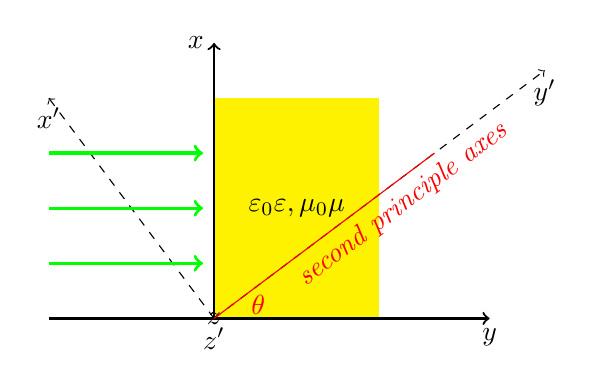
\begin{tikzpicture}[xscale=0.7, yscale=0.7]
    %-------------------- anisotropic slab --------------------------------------------------------    
        \fill[fill=yellow] (2,0) rectangle (5,4)node [pos=0.5]{$\varepsilon_0 \boldsymbol \varepsilon, \mu_0 \boldsymbol\mu $};
    %-------------------------- coordinate--------------------------------------------
         \draw [->,thick] (2,0) node{$z$} -- (2,5.0) node[left]{$x$} ;
         \draw [->,thick] (-1,0) -- (7,0) node [below]{$y$};
    %------------------------- principle axes of the media ------------------------------------
        \draw [-> ,dashed] (2,0)node [below]{$z^{\prime}$} -- (8,4.5)  node [below]{$y^{\prime}$};
    \draw [-> ,dashed] (2,0) -- (-1,4) node [below]{$ x^{\prime}$};
    %---------------------------third optical axes-------------------------------------------    
       \draw [red] (2,0) -- (6,3) node [pos=0.2, below]{$\theta$} node [pos=.8, below, rotate=37]{\textit{second principle axes}} ;              
    %-------------------------- light rays-------------------------------------------------------
        \draw [-> , green,very thick] (-1,1)  -- (1.8,1)  ;
        \draw [->,green,very thick] (-1,2)  -- (1.8,2) ;
        \draw [->,green,very thick] (-1,3)  -- (1.8,3)  ;            
    \end{tikzpicture}
\caption{Schematic of an anisotropic slab with $\boldsymbol{\varepsilon}$ and $\boldsymbol{\mu}$ as a tensor, light incidents from left and propagation plane is $y-z$ plane; two principle axes of media  $z^{\prime}$ and $y^{\prime}$ do not lay on the $z$ and $y$ coordinate.}
    \label{figure1}
\end{figure}
\section{ Method}

We are determining the optical metric, of a medium, perceived by passing light from the eikonal equations.
For this purpose, we write an eikonal equation of the rays in the empty curved space-time. A comparison between eikonal equations in arbitrary curved space-time and those in the anisotropic medium (in Cartesian coordinate) indicated that the coefficients of the eikonal equations can be interpreted as a component of the $\mathbf{g}^{-1}$, i.e. the inverse metric of the effective geometry. 
This method can be applied to finding the effective geometry for all kind of anisotropic media.

In the non-magnetic anisotropic medium, the tensorial form of the electric permittivity results in two dispersion surfaces (eikonal equations) for each propagation direction of the electromagnetic waves \cite{born1999principles}. 
These dispersion surfaces specify two independent directions of the polarization as a normal mode of the medium. An arbitrary polarization light in these media can be considered as a superposition of these two independent normal modes \cite{saleh1991fundamentals}.
 Each normal mode is associated with a different refractive index, and therefore, perceives its geometry.  In the non-magnetic medium, unlike the impedance-matched media, we cannot associate a unique metric to the medium, while the metric is strongly depends on the angle of incident.
We fond that the light with out-of-plane polarization," TE polarization",  is one of the normal modes that perceives non-magnetic media as an isotropic response from the medium, whereas the light with in-plane polarization "TM polarization," sees the anisotropic response. 



\subsection{geometrical optics regime}

In the inhomogeneous electromagnetic media, a general solution of the Maxwell equations can be approximated to a quasi plane wave with slowly varying amplitude and fast oscillating phase, while geometrical optics limits are valid \cite{kravtsov1990geometrical, sluijter2010ray, leonhardt2012geometry}, 

\begin{gather} \label{general-sl}
\{\mathbf{E,H}\}(\mathbf{r},t)=\{\mathbf{E,H}\}(\mathbf{r})e^{-i\varphi(\mathbf{r},t)}
\end{gather}
\begin{equation}\label{geometric-optic}
\nabla{\varphi(r,t)}\gg 1,\qquad E(\mathbf{r})\approx constant.
\end{equation}

where the wave vector $\mathbf{k}$ and the angular frequency $\omega$  are defined as

\begin{equation}
\mathbf{k}=\nabla{\varphi(r,t)} \qquad
\omega=-\dfrac{\partial{\varphi(r,t)}}{\partial{t}}.
\label{wave}
\end{equation}

In this paper we assume that the phase is not depend on the time explicitly; So the phase of the wave takes the following form:
\begin{equation}
\varphi(\mathbf{r},t)=\int{\mathbf{k}\cdot \mathrm{d}\mathbf{r}}-\omega {t}
\end{equation}
Compared with the plane wave in the vacuum, $k_{0}\cdot \mathrm{d}\mathbf{r}-\omega t $, we can write the phase as
\begin{equation}
\varphi(\mathbf{r},t)=k_{0}\psi(\mathbf{r})-\omega t ,
\end{equation}
where ,$\psi(\mathbf{r})$ 
\begin{equation}
\psi(\mathbf{r}):=\frac{1}{k_{0}}\int{\mathbf{k}\cdot \mathrm{d}\mathbf{r}}.
\end{equation}
is called eikonal.  Using phase refractive index, $n_{p}=k/k_{0}$, \cite{born1999principles}, we can write the eikonal as 
\begin{equation}
\psi(\mathbf{r})=\int{n_{p}\hat{U}\cdot \mathrm{d}\mathbf{r}}.
\end{equation}
where the unit vector, $\hat{U}$ is along the wave vector direction. 
Therefore, the eikonal, $\psi(\mathbf{r})$, is a function of the optical path length.\\


\subsection{Inhomogeneous anisotropic media}

Maxwell's equations in anisotropic charge-free and current-free materials, $\rho=0, \quad \mathbf{J}=0 $,   are given by \cite{born1999principles},

\begin{gather}
\nabla\cdot \mathbf{D} =0,\quad \nabla\cdot \mathbf{B} =0, \nonumber \\
\nabla\times\mathbf{E}=-\dfrac{\partial\mathbf{B}}{\partial t}, \quad \nabla\times\mathbf{H} =-\dfrac{\partial\mathbf{D}}{\partial t}.\label{m.h}
\end{gather}
We consider the constitutive equations for the anisotropic material as
 \begin{equation} 
 \mathbf {D}=\varepsilon_0 \boldsymbol \varepsilon \mathbf{E},  \qquad
  \mathbf{B}=\mu_0 \boldsymbol\mu \mathbf{H},
  \end{equation}
where $\boldsymbol{\varepsilon}$ and $\boldsymbol{\mu}$  are the electric permittivity and  the magnetic permeability tensors respectively. 


Using the quasi planewave (\ref{general-sl}) as a general solution, the Maxwell equation can be written as 
\begin{gather}
\boldsymbol{\nabla}{\psi}\cdot\mathbf{D}=-\dfrac{1}{ik_{0}}\boldsymbol{\nabla}\cdot \mathbf{D}, \nonumber\\
\boldsymbol{\nabla}{\psi}\cdot \mathbf{B}=-\dfrac{1}{ik_{0}}\boldsymbol{\nabla}\cdot \mathbf{B},\nonumber\\
\boldsymbol{\nabla}{\psi}\times\mathbf{E}-c\mathbf{B}=-\dfrac{1}{ik_{0}} \boldsymbol{\nabla}\times\mathbf{E},\nonumber\\
\boldsymbol{\nabla}{\psi}\times\mathbf{H}-c\mathbf{D}=-\dfrac{1}{ik_{0}} \boldsymbol{\nabla}\times\mathbf{H},\label{m.i}
\end{gather}
where $c={1}/{\sqrt{\mu_{0}\varepsilon_{0}}}$.

In geometrical optics regime, (\ref{geometric-optic}), we have $k_{0}\gg1$; So, the right-hand side of the above equations (\ref{m.i}) can be neglected.  Therefore, the wave equation can be obtained as 

\begin{eqnarray}
\boldsymbol{\nabla}{\psi}\times{\boldsymbol{\mu^{-1}}(\boldsymbol{\nabla}{\psi}\times\mathbf{E})}=-\boldsymbol{\varepsilon}\mathbf{E}.
\end{eqnarray}
By using $\nabla{\psi}=k/k_{0}$, the wave equation in inhomogeneous anisotropic media, similar to  the wave equation in homogeneous anisotropic material, take the following form: 

\begin{eqnarray}\label{wave equations}
\mathbf{k} \times{\boldsymbol{\xi}(\mathbf{k}\times\mathbf{E})}=-k^{2}_{0}\boldsymbol{\varepsilon}\mathbf{E},
\end{eqnarray}
where $\boldsymbol{\xi}=\boldsymbol{\mu}^{-1}$. 
We can rewrite the equation (\ref{wave equations}) in a matrix form as
\begin{equation}\label{matrix form}
\mathbf{M}\mathbf{E}=-k_{0}^{2}\boldsymbol{\varepsilon}\mathbf{E}, . 
\end{equation}
This matrix equation has a non-trivial solution, if the determinant of the coefficients vanishes,
\begin{equation}\label{eikonal-e}
\mathrm{det}(\mathbf{M}+k_{0}^{2}\boldsymbol{\varepsilon})=0
\end{equation}
This equation, (\ref{eikonal-e}), can be rewritten as
\begin{equation}\label{eikonal-eq}
G_{1}(k^2,k^2_{0})G_{2}(k^2,k^2_{0})=0
\end{equation}

$G_{1}=0$ and $G_{2}=0$ are the solution of this equation, (\ref{eikonal-eq}), which is named the dispersion relation; 

According to the relation $\mathbf{k}=\nabla{\varphi(r,t)}$, in geometric optics, these relations are called eikonal equations. 

On the other hand, these equations $G_{1}=0$ and $G_{2}=0$ can be considered as the Hamiltonian of the light in the anisotropic medium,\cite{schurig2006calculation, sluijter2008general}, 
\begin{eqnarray}
H_{1}=f(r)G_{1}(k^2,k^2_{0}) \qquad H_{2}=f(r)G_{2}(k^2,k^2_{0})
\end{eqnarray}
The ray tracing is performed by solving the Hamiltonian equations,
\begin{eqnarray}\label{hamilton}
\dfrac{\mathrm{d}x_{i}}{\mathrm{d}t}=\dfrac{\partial{H}}{\partial{k_{i}}}\\
\dfrac{\mathrm{d}k_{i}}{\mathrm{d}t}=-\dfrac{\partial{H}}{\partial{x_{i}}}
\end{eqnarray}

\subsection{wave equation in curved space}
Electromagnetic wave equation in curved vacuum space is given by
\begin{equation}\label{c-wave}
\nabla^{j} \nabla_{j} E_{i} - R_{ij}E^{j}-\dfrac{1}{c^2} \dfrac{\partial^{2}E_{i}}{{\partial t}^{2}}=0
\end{equation}
where $R_{ij}$ is a Riemann curvature tensor. In general, the  Riemann curvature tensor is given by \cite{leonhardt2012geometry}
\begin{equation}\label{Riemann}
R^{i}_{jkl}\equiv \Gamma^{i}_{jl,k}-\Gamma^{i}_{jk,l}+\Gamma^{i}_{mk}\Gamma^{m}_{jl}-\Gamma^{i}_{ml}\Gamma^{m}_{jk}
\end{equation}

where $\Gamma^{i}_{jk}$ are Christoffel symbols and the comma notation "$,$" refers to partial differentiation.  The Christoffel symbols are expressed in terms of the metric components,
\begin{equation}\label{cr}
\Gamma^{i}_{jk}=\dfrac{1}{2} g^{il}(g_{lj,k}+g_{lk,j}-g_{jk,l})
\end{equation}
Using quasi planewave(\ref{general-sl}) the wave equation (\ref{c-wave}) can be written as \cite{leonhardt2012geometry}
\begin{equation}
\begin{split}
&\nabla^{j}\nabla_{j}E_{i}+2i(\nabla_{j}E_{i})\nabla^{j}{\phi(r,t)}-
(\nabla^{j}{\phi(r,t)})(\nabla_{j}{\phi(r,t)})E_{i}\\
 &+i(\nabla^{j}\nabla_{j}{\phi(r,t)})E_{i} + \nabla^{j}\nabla_{i}E_{i} -R_{ij}E^{j}  \\
&-\dfrac{1}{c^2}\left(\dfrac{\partial^2 E_{i}}{\partial t^2}-2i(\dfrac{\partial\phi(r,t)}{\partial t})(\dfrac{\partial E_{i}}{\partial t})-(\dfrac{\partial\phi(r,t)}{\partial t})^2 E_{i}\right)=0
\end{split}
\end{equation}

In geometric optics, (\ref{geometric-optic}), above relation reduces to

\begin{equation}
\left(k^{j}k_{j}-i(\nabla^{j}k_{j})+ \dfrac{\omega^2}{c^2} \right) E_{i}+R_{ij}E^{j}=0
\end{equation}
where $k^{j}=\nabla^{j}{\phi(r,t)}$ and $k_{j}=\nabla_{j}{\phi(r,t)}$
For quasi plane wave to be a good approximation, we need, \cite{leonhardt2012geometry},
\begin{equation}
\nabla^{j}k_{j}\ll 1, \qquad  \mid{R_{ij}}\mid \ll \mid{k}\mid
\end{equation}
Therefore, Eikonal equation for the electromagnetic waves in empty curved space-time in geometric optics limit take the following form:
 
\begin{equation}\label{dispersion}
g^{\mu\nu}k_{\mu}k_{\nu}=0
\end{equation}
where $g^{\mu\nu}$ is the inverse of the space-time metric and $k_{0}={\omega}/{c}$.

As it mentioned  previously, we can choose eikonal equation (\ref{dispersion}) as the Hamiltonian of the light,
\begin{equation}
H=g^{\mu\nu}k_{\mu}k_{\nu}.
\end{equation}
Using Hamiltonian equations, (\ref{hamilton}), the group velocity of the light can be obtained as
\begin{eqnarray}\label{group}
\dfrac{\mathrm{d}x^{i}}{\mathrm{d}t}=g^{ij}k_{j}=k^{i}.
\end{eqnarray}
Group velocity indicate the ray direction in media; So we can see the ray direction in the curved space-time differ from wave vector, $k_{i}$, and it is along the contravariant vector $k^{i}$.

 \section{Analogy between curved space-time and anisotropic medium}
 
According to the subjects mentioned in the previous section, we can find  the effective geometry perceived by light in Anisotropic media via two following methods:

First, by a comparison between the eikonal equations of the light in media, (\ref{eikonal-eq}), and in the curved space-time, (\ref{dispersion}). With notice to the relation (\ref{eikonal-eq}), we can rewrite the relations $G_{1}(k^2,k^2_{0})=0$ and $G_{2}(k^2,k^2_{0})=0 $, the eikonal equations of the each normal mode of the anisotropic media, as $g_{1}^{\mu\nu}k_{\mu}k_{\nu}=0$, and $g_{2}^{\mu\nu}k_{\mu}k_{\nu}=0$; Then by comparing with the (\ref{dispersion}), eikonal equation of the light in empty space-time, we find that the $g_{1}^{\mu\nu}$  and $g_{2}^{\mu\nu}$  are the inverse metrics of the effective geometry that the each normal mode perceives in birefringent media.  
However, some detailed hints should be considered in the use of these methods.

Second, usage of the wave vector and ray vector of the light in the medium.
According to the relation (\ref{group}), we can rewrite this relation as 
\begin{equation}\label{direction}
\mathbf{v}_{ray}=g^{-1}\mathbf{k}
\end{equation}
So, The only thing we have to do is to find a transformation matrix that related ray vector to the wave vector.

 
\subsection{The anisotropic medium seen as the isotropic medium}\label{isotropic-a}

We can find the effective metric of the medium by a comparison between line element of the optical path in medium and empty curved space-time \cite{ }. 
By applying this method, we find conformally flat spaces that light perceives in the medium.

According to the Fermat principle, optical path length in the medium(OPL) given by

\begin{equation}\label{opl}
OPL=\int{ndl}
\end{equation}
where $n$ is the refractive index along the the line element $dl$. In anisotropic media, the ray direction can be different from the wave vector; Therefore the refractive index $n$ appeared in (\ref{opl}) refers to the ray refractive index, $n_{ray}$. Using definition of the ray refractive index, $n_{r}^{2}=\frac{dl_{vaccum}^{2}}{dl_{medium}^{2}}$, and the line element in curved space, $ dl_{vaccum}^{2}=g_{ij}dx^{i}dx^{j}$, we can find the ray refractive index as
\begin{equation}\label{ray1}
n_{r}^{2}=\dfrac{g_{ij}dx^{i}dx^{j}}{dl^{2}}
\end{equation}
if we define the angle between $dx^{j}$ and $dl$ by $\alpha_{j}$ as
\begin{equation}
\cos{\alpha^{j}}=\dfrac{dx^{j}}{dl}
\end{equation}
Then we can rewrite relation (\ref{ray1}) as
\begin{equation}\label{nray}
n_{r}^{2}=g_{ij}\cos{\alpha^{j}}\cos{\alpha^{i}}
\end{equation}

As we can see from above, we find the refractive index of the equivalent inhomogeneous isotropic medium that light feels through passing inhomogeneous, Anisotropic medium. 
We can establish an analogy between the isotropic medium and the anisotropic medium for each normal modes of the anisotropic medium.

\section{Effective geometry of the planar media}\label{planar media}

In this section, we use above mentioned method to investigating dielectric media that has the dielectric permittivity tensor as

\begin{align}\label{planar1}
        \boldsymbol{\varepsilon}=
        \begin{pmatrix}
             \varepsilon_{11} &\varepsilon_{12} &0 \\
            \varepsilon_{21}&\varepsilon_{22}  &0\\
            0&0 &\varepsilon_{33}
        \end{pmatrix}.
\end{align}
because this dielectric tensor has a non-diagonal in two direction, we name these kind of media as a planar media.
For obtaining the eikonal equation, we must first obtain the $\mathbf{M}$  matrix in the relation (\ref{eikonal-e}). 
Without any restrictions on the permeability of the medium, the component of the matrix $\mathbf{M}$ can obtained through the following relations:

\begin{align}
M_{11}&=2\xi_{23}k_{z}k_{y}-(\xi_{33}k_{y}^{2}+\xi_{22}k_{z}^{2}), \nonumber\\
M_{12}&=\xi_{21}k_{z}^{2}-\xi_{23}k_{z}k_{x}-\xi_{31}k_{z}k_{y}+\xi_{33}k_{y}k_{x}, \nonumber\\
M_{13}&=\xi_{31}k_{y}^{2}-\xi_{23}k_{y}k_{x}-\xi_{21}k_{z}k_{y}+\xi_{22}k_{z}k_{x}, \nonumber\\
M_{22}&=2\xi_{13}k_{z}k_{x}-(\xi_{33}k_{x}^{2}+\xi_{11}k_{z}^{2}), \nonumber\\
M_{23}&=\xi_{32}k_{x}^{2}-\xi_{12}k_{z}k_{x}-\xi_{31}k_{y}k_{x}+\xi_{11}k_{y}k_{z},\nonumber\\
M_{33}&=2\xi_{21}k_{x}k_{y}-(\xi_{22}k_{x}^{2}+\xi_{11}k_{y}^{2}).
\end{align}
Where $\boldsymbol{\xi}=\boldsymbol{\mu}^{-1}$. 



 Also, for simplicity, we consider the $x-y$ plane as  the incident plane, Fig, \ref{figure1} . Therefore the $z$ component of the wave vector is zero, $k_{z}=0$. In applying this assumption we must care. we can apply this assumption after the determination of the ray direction. Nevertheless, Because the permittivity tensor has the planar form, (\ref{planar1}), the ray direction also lies in the $x-y$ plane and therefore we can apply above assumption, $k_x=0$, to the $\mathbf{M}$ matrix, 
 \begin{align}\label{m}
M_{11}&=-\xi_{33}k_{y}^{2}, \nonumber\\
M_{12}&=\xi_{33}k_{y}k_{x}, \nonumber\\
M_{13}&=\xi_{31}k_{y}^{2}-\xi_{23}k_{y}k_{x}, \nonumber\\
M_{22}&=-\xi_{33}k_{x}^{2}, \nonumber\\
M_{23}&=\xi_{32}k_{x}^{2}-\xi_{31}k_{y}k_{x},\nonumber\\
M_{33}&=2\xi_{21}k_{x}k_{y}-(\xi_{22}k_{x}^{2}+\xi_{11}k_{y}^{2}).
\end{align}

 Also, we  study two important case of electromagnetic medium: First, the anisotropic medium in impedance matching with the vacuum, $\boldsymbol{\varepsilon}=\boldsymbol{\mu}$ called impedance-matched anisotropic medium and second, the anisotropic medium with electric anisotropy, $\mu=1$, that we call it "Electric Medium."  
 
 \subsection{Impedance-matched media}
We assume the anisotropic media with the the permittivity tensor (\ref{planar1}) became in impedance-matching with the vacuum, $\boldsymbol{\mu}=\boldsymbol{\varepsilon}=(\ref{planar1})$. So we can write
\begin{equation}
\boldsymbol{\xi}=\boldsymbol{\varepsilon}^{-1}=\frac{1}{\varepsilon_{1} \varepsilon_{2}}
        \begin{pmatrix}
             \varepsilon_{22} &-\varepsilon_{12} &0 \\
            -\varepsilon_{21}&\varepsilon_{11}  &0\\
            0&0 &\frac{\varepsilon_{1} \varepsilon_{2}}{\varepsilon_{3}}
        \end{pmatrix}.
\end{equation}

Therefore, the components of the $\mathbf{M}$ matrix are reduced to 
\begin{align}\label{m1}
M_{11}&=-\dfrac{1}{\varepsilon_{3}} k_{y}^{2}, \nonumber\\
M_{12}&=\dfrac{1}{\varepsilon_{3}}k_{y}k_{x}, \nonumber\\
M_{13}&=0, \qquad M_{23}=0,\nonumber\\
M_{22}&=-\dfrac{1}{\varepsilon_{3}}k_{x}^{2}, \nonumber\\
M_{33}&=\frac{1}{\varepsilon_{1} \varepsilon_{2}}\left(-2\varepsilon_{21}k_{x}k_{y}-\varepsilon_{11}k_{x}^{2}-\varepsilon_{22}k_{y}^{2}\right).
\end{align}

Substituting the relations (\ref{m1}) and (\ref{planar1}) in equation (\ref{eikonal-e}), we obtain equation (\ref{eikonal-eq}), $G_{1}(k^2,k^2_{0})G_{2}(k^2,k^2_{0})=0$ as
\begin{eqnarray}
G_{1}=-\varepsilon_{1}\varepsilon_{2} k_{0}^{2}+\dfrac{1}{\varepsilon_{3}} \left(\varepsilon_{11}k_{x}^{2}+\varepsilon_{22}k_{y}^{2}+2\varepsilon_{12}k_{x}k_{y}\right)=0 \label{dispersion-imp1}\\ 
G_{2}=\varepsilon_{3} k_{0}^{2}-\dfrac{1}{\varepsilon_{1}\varepsilon_{2}}\left(\varepsilon_{11} k_{x}^{2}+\varepsilon_{22}k_{y}^{2}+2\varepsilon_{12}k_{x}k_{y}\right)=0
\label{dispersion-imp2}
\end{eqnarray}

As pointed in previous section, the coefficient of the eikonal equations can be interpreted as the components of the $\mathbf{g}^{-1}$, where $\mathbf{g}$ is the metric tensor of the effective geometry perceived by light. So we can find two metrics as
\begin{gather}
\mathbf{g}^{-1}_{1}(1+2)=
\begin{pmatrix}
-\varepsilon_{1}\varepsilon_{2}&0&0\\
0&\dfrac{\varepsilon_{11}}{\varepsilon_{3}}& \dfrac{\varepsilon_{12}}{\varepsilon_{3}}\\
0&\dfrac{\varepsilon_{12}}{\varepsilon_{3}}&\dfrac{\varepsilon_{22}}{\varepsilon_{3}}
\end{pmatrix}, \label{m1-imp} \\
\mathbf{g}^{-1}_{2}(1+2)=
\begin{pmatrix}
-\varepsilon_{3}&0&0\\
0&\dfrac{\varepsilon_{11}}{\varepsilon_{1}\varepsilon_{2}}& \dfrac{\varepsilon_{12}}{\varepsilon_{1}\varepsilon_{2}}\\
0&\dfrac{\varepsilon_{12}}{\varepsilon_{1}\varepsilon_{2}}&\dfrac{\varepsilon_{22}}{\varepsilon_{1}\varepsilon_{2}}
\end{pmatrix},
\end{gather}
Two above metrics  are conformally equivalent. Indeed, Expressions (\ref{dispersion-imp1}) and (\ref{dispersion-imp2}) are equivalent. Therefore, in impedance matched anisotropic medium we have only one eikonal equation; these kind of media are not birefringence. Precisely in the above eikonal equations, (\ref{dispersion-imp1}) and (\ref{dispersion-imp2}), we find the following form for the component of the $\mathbf{g}^{-1}$:
\begin{eqnarray}\label{m-imp}
\dfrac{g^{ij}}{g^{00}}=-(\det{\boldsymbol{\varepsilon}})^{-1}\varepsilon^{ij}
\end{eqnarray}
where $\det{\boldsymbol{\varepsilon}}=\varepsilon_{1}\varepsilon_{2}\varepsilon_{3}$ and $i,j=1,2$. This relation, (\ref{m-imp}), specifies the (2+1) space-times that are conformally equivalent together. If we choose $g_{00}=1$  the effective metric become:
\begin{align}\label{m2-imp}
\mathbf{g}_{imp}(2+1)=
\begin{pmatrix}
-1&0&0\\
0&\varepsilon_{3}\varepsilon_{22}& -\varepsilon_{3}\varepsilon_{12}\\
0&-\varepsilon_{3}\varepsilon_{12}&\varepsilon_{3}\varepsilon_{11}
\end{pmatrix},
\end{align}

As an important point, above results, ( \ref{m-imp}) and (\ref{m2-imp}), are in agreement with the metrics has achieved in the \cite{leonhardt2012geometry}. Therefore, our method achieved in geometrical optics limit is verified. 

\subsection{Non-magnetic media}

For the case of the electric media, $\boldsymbol{\mu}=1$,  therefore the components of the $\mathbf{M}$ matrix can be written as
\begin{align}\label{m2}
M_{11}&=-k_{y}^{2}, \nonumber\\
M_{12}&=k_{y}k_{x}, \nonumber\\
M_{13}&=0, \qquad M_{23}=0,\nonumber\\
M_{22}&=-k_{x}^{2}, \nonumber\\
M_{33}&=-k_{x}^{2}-k_{y}^{2}.
\end{align}
If we consider the permittivity tensor as (\ref{planar1}), The two eikonal equations, $G_{1}=0$ and $G_{2}=0$ can be obtained as
\begin{eqnarray}
&G_{1}(k^2,k^2_{0})=-k^{2}_{0} \varepsilon_{33}+(k_{x}^{2}+k_{y}^{2})=0 \label{out}\\
&G_{2}(k^2,k^2_{0})=-\varepsilon_{1}\varepsilon_{2} k_{0}^{2}+\varepsilon_{11}k_{x}^{2}+\varepsilon_{22}k_{y}^{2}+2\varepsilon_{12}k_{x}k_{y}=0 \label{in}
\end{eqnarray}
Two different eikonal equations point to the birefringent effect in these media. The value of the $ k_{x}$ is determined from the phase matching condition on the boundary. For every $k_{x}$, solving dispersion relations (\ref{out}) and (\ref{in}), we can find four solutions for the $k_{y}$ as $\pm k_{y1}$ and $\pm k_{y2}$ where the $-k_{y1}$ and $-k_{y2}$ is concerned to the refractive rays. In this paper, we consider the  $+kـ{y1}$ and $+k_{y2}$ which are concerned to the transmitted rays. 

Solving the eikonal equation (\ref{out}),  shows this equation (\ref{out}) is concerned to the light with out-of-plane polarization,TE polarization polarization, whereas the eikonal equation (\ref{in}) is concerned to the light with in-plane polarization, TM polarization.For both the TE and TM polarization, according to the eikonal equations, effective geometry is a $(2+1)$ space-time, but they perceive different geometry in this media.

For the TE polarization, Inverse matrix of the metric tensor can be written as $g^{ij}=\frac{g^{00}}{\varepsilon_{33}}\delta^{ij}$. If we choose $g^{00}=\varepsilon_{33}$, the effective metric for the TE light given by

\begin{align}\label{metric-te}
\mathbf{g}^{TE}(2+1)=
\begin{pmatrix}
-\dfrac{1}{\varepsilon_{3}}&0&0\\
0&1& 0\\
0&0&1
\end{pmatrix}
\end{align}
This metric is conformally equivalent with the effective geometry of the two dimensional isotropic media that its refractive indexes is $n=\sqrt{\varepsilon_{33}}$. 
For the TM polarization, Inverse matrix of the metric tensor can be written as

 \begin{equation}
g^{ij}=\dfrac{g^{00}}{\varepsilon_{1}\varepsilon_{2}}\varepsilon^{ij}
\end{equation}

Therefore, if we set the $g^{00}=1$ then TM polarization feels this planar media (\ref{planar1}) as space-time with the following metric: 

\begin{align}\label{metric-tm}
\mathbf{g}^{TM}(2+1)=
\begin{pmatrix}
-1&0&0\\
0&\varepsilon_{11}& \varepsilon_{12}\\
0&\varepsilon_{12}&\varepsilon_{22}
\end{pmatrix} 
\end{align}
Hence, the electric planar media  for each  eigen-polarizations of the medium, in our case TE and TM polarization, appear as two distinct space-time. We can apply this property for designing multi functional devices based on transformation optics.

\subsection{Non-magnetic anisotropic medium as an alternative to the impedance-matched medium } 

In the previous subsections, we obtain the effective metrics felled by light in the impedance matching and electric media. Now we want to establish relation between these effective space-times. For this aim, the comparison between the metrics (\ref{metric-te}), (\ref{metric-tm}) and (\ref{m1-imp}) show the metric $\mathbf{g}^{imp}(2+1)$ is similar to the $\mathbf{g}^{TM}(2+1)$. For better comparison between these metrics, we rewrite the planar permittivity tensor (\ref{planar1}) as
\begin{equation}\label{planar2}
\boldsymbol{\varepsilon}=
        \begin{pmatrix}         
            \boldsymbol{\varepsilon}_{p}  &0\\
            0&\varepsilon_{33}        
        \end{pmatrix}.
\end{equation}

where $\boldsymbol{\varepsilon}_{p}$ is the permittivity of the medium in the $x-z$ plane,
\begin{align}\label{t-per}
        \boldsymbol{\varepsilon}_{p}=
        \begin{pmatrix}         
            \varepsilon_{11}  &\varepsilon_{12}\\
            \varepsilon_{12} &\varepsilon_{22}
        \end{pmatrix}.
\end{align}
Also, according to form of the metrics (\ref{metric-tm}) and (\ref{m1-imp}), we can rewrite $\mathbf{g}^{imp}$ and $\mathbf{g}^{TM}$ as

\begin{eqnarray}\label{m-imp}
\mathbf{g}^{imp}=
        \begin{pmatrix}         
            -g^{imp}_{00}     &0\\
            0&\mathbf{g}^{imp}_{p}
        \end{pmatrix} \qquad
    \mathbf{g}^{TM}=
        \begin{pmatrix}         
            -g_{00}^{TM}&0\\
            0&\mathbf{g}^{TM}_{p}
        \end{pmatrix}.
\end{eqnarray}
where the $\mathbf{g}^{imp}_{p}$ and $\mathbf{g}^{TM}_{p}$ are  the spatial part of the (\ref{metric-tm}) and (\ref{m1-imp}), the two dimensional effective geometry felt by light through the passing medium. Therefore, according to the relation (\ref{m-imp} and the eikonal equation (\ref{out}),we obtain $\mathbf{g}^{imp}_{p}$ and $\mathbf{g}^{TM}_{p}$ as

\begin{eqnarray}
\mathbf{g}^{imp}_{p}=g^{imp}_{00}(\det{\boldsymbol{\varepsilon}})\boldsymbol{\varepsilon}^{-1}_{p}
\label{gimp}\\
\mathbf{g}^{TM}_{p}=g^{TM}_{00}(\det{\boldsymbol{\varepsilon}}_{p})\boldsymbol{\varepsilon}_{p}^{-1}
\label{gtm}
\end{eqnarray}
These metric are conformally equivalent; If we assume
\begin{equation}\label{eq-cond}
g^{TM}_{00}=g^{imp}_{00}\varepsilon_{33}
\end{equation}
these metrics be came equivalent, $\mathbf{g}^{TM}_{p}=\mathbf{g}^{imp}_{p}$. Consequently, the effective spatial geometry felt by TM polarization in the Electric media is equivalent with the one perceived by light in impedance-matched anisotropic media; The only difference between them are concerned to the their perception of the time. The condition (\ref{eq-cond}) shows the TM polarized light in electric medium passing through this effective space faster than the light in impedance-matched medium, $\mathbf{v}^{TM}=\varepsilon_{33}\mathbf{v}^{imp}$, where $\mathbf{v}$ is the velocity of light.
Also we can verify these similarity between the effective geometries, $\mathbf{g}^{imp}_{p}$ and $\mathbf{g}^{TM}_{p}$, by finding the direction of the light in these medium as the geodesics of these effective geometries. For this work, we consider the Hamiltonian of the ray, (\ref{hamilton}), in  impedance-matching and electric medium as
 \begin{eqnarray}
H^{imp}=-\varepsilon_{1}\varepsilon_{2}\varepsilon_{3} k_{0}^{2}+\varepsilon_{11}k_{x}^{2}+\varepsilon_{22}k_{y}^{2}+2\varepsilon_{12}k_{x}k_{y}\\
H^{TM}=-\varepsilon_{1}\varepsilon_{2} k_{0}^{2}+\varepsilon_{11}k_{x}^{2}+\varepsilon_{22}k_{y}^{2}+2\varepsilon_{12}k_{x}k_{y}
\end{eqnarray}
Using Hamilton equation, 
\begin{equation}
\dfrac{\mathrm{d}q_{i}}{\mathrm{d}t}=\dfrac{\partial{H}}{\partial{k_{i}}}
\end{equation}
we find
\begin{eqnarray}\label{direction}
\left(\dfrac{\mathrm{d}x}{\mathrm{d}y}\right)^{TM}=\left(\dfrac{\mathrm{d}x}{\mathrm{d}y}\right)^{imp}=\dfrac{\varepsilon_{11}k_{x}+\varepsilon_{12}k_{y}}{\varepsilon_{22}k_{y}+\varepsilon_{12}k_{x}}
\end{eqnarray}
The direction of the light propagation in the impedance matched anisotropic medium is same with the direction of the TM polarized light in the Electric medium. We know, the light trajectory is the geodesics of the effective geometry, therefore relation (\ref{direction}) verifies that these effective geometries are equivalent together.

As a supplementary point, relation (\ref{direction}) also indicated that the direction of the light in impedance-matched media as well as TM light in Electric media do not along the direction of the wave vector, $\mathbf{K}$, they are indeed extraordinary light whereas the direction of the TE light in the electric medium is along the wave vector and is ordinary light.
\begin{eqnarray}
&H^{TE}=-k^{2}_{0} \varepsilon_{33}+(k_{x}^{2}+k_{y}^{2})\\
&\left(\dfrac{\mathrm{d}\mathbf{r}}{\mathrm{d}r}\right)^{TE}=\dfrac{\mathbf{k}}{k}
\end{eqnarray}

This analogy between planar impedance-matching anisotropic media and planar Electric media in respond to the in-plane polarized light is a very useful especially for the analog gravity field.

As some examples, we refer to the articles:\cite{chen2010transformation}, "Transformation optics that mimics the system outside a Schwarzschild black hole", \cite{lai2009complementary}, "Complementary media invisibility cloak that cloaks objects at a distance outside the cloaking shell."

In all these cases the impedance-matched anisotropic media obtained in these articles, have a planar form of the permittivity and permeability. Therefore according to the above mention calculation, we can realize these novel optical devices by using non-magnetic media in respond to the TM polarized light.

\subsection{Planar media as conformally flat spaces for the light in $y-z$ plane}
Also according to the \ref{isotropic-a}, we have
\begin{align}
\mathbf{g}(2+1)=
\begin{pmatrix}
-1&0&0\\
0&n_{r}^{2}& 0\\
0&0&n_{r}^{2}
\end{pmatrix}.
\end{align}
by finding the ray refractive indexes, we can find  isotropic inhomogeneous media in analogous with this planar electric media and impedance-matched planar media.
Substituting (\ref{gimp}) and (\ref{gtm}) in (\ref{nray}), The ray refractive index for travelling wave in the $x-y$ plane obtained as

\begin{equation}\label{g-nray}
n_{r}^{2}=C\Sigma_{ij} (\boldsymbol{\varepsilon}_{p}^{-1})_{ij}\cos{\alpha}_{ij}
\end{equation}
where $C$ is $g^{imp}_{00}(\det{\boldsymbol{\varepsilon}})$ in impedance matched media or $g^{imp}_{00}(\det{\boldsymbol{\varepsilon}_{p}})$ in electric media. In the $x-y$ plane, if we consider $dy/dl=\cos{\phi}$ So $dx/dl=\sin{\phi}$ then the relation(\ref{direction}) can be written as
\begin{equation}
\tan{\phi}=\dfrac{\varepsilon_{11}k_{x}+\varepsilon_{12}k_{y}}{\varepsilon_{22}k_{y}+\varepsilon_{12}k_{x}}
\end{equation}

Therefore, we obtain the ray refractive index, \ref{g-nray} as
\begin{equation}\label{f-nray}
n_{r}^{2}=C(\varepsilon_{22}\sin{\phi}^{2} +2\varepsilon_{12}\sin{\phi}\cos{\phi} +\varepsilon_{11}\cos{\phi}^{2})
\end{equation}
Consequently, light  perceive Electric medium as conformally flat spaces with the above refractive index, (\ref{f-nray})

\section{Medium with variable optical axes}

The plenary permittivity tensors of the form (\ref{planar1}) reveals that third principle axis, $z^{\prime}$, leis along the $z$ axis, whereas the two other principle axes of the medium, $x^{\prime}, y^{\prime}$ do not lei on the $x$ and $y$ axes but they has rotated and lie in the $x-y$ plane such as Fig. \ref{figure1}. Therefore, this form of tensor, (\ref{planar1}), follows the relation \cite{yeh1980optics},

 \begin{eqnarray}\label{t.t}
        \boldsymbol{\varepsilon}= \mathbf{A} \boldsymbol{\varepsilon^{\prime}}\mathbf{A}^{T},
        \end{eqnarray}
where $ \boldsymbol{\varepsilon^{\prime}} = \mbox{diag} (\varepsilon_{1},\varepsilon_{2},\varepsilon_{3})$ and $\boldsymbol{\mu^{\prime}} = \mathrm{diag} (\mu_{1},\mu_{2},\mu_{3}) $  are  principle dielectric tensors and $\mathbf{A}$  is the rotation matrix, which describes the rotation of the coordinate axes with respect to the crystal principle axes and $ \mathbf{A}^{T}$ is transpose of the rotation matrix $ \mathbf{A}$. 


Therefore, the rotation matrix $\mathbf{A}$ according to the Fig. \ref{figure1} is given by
 
\begin{align}\label{r.m}
        \mathbf{A}=\mathbf{R}_{x}(\theta)=
        \begin{pmatrix}            
            \cos{\theta} &\sin{\theta}&0 \\
            -\sin{\theta} & \cos{\theta}&0\\
            0&0&1
        \end{pmatrix},
\end{align}
where $\theta$ is a angle between $y$ and $y^{\prime}$.  So, using Eq. (\ref{t.t}),  we can obtain the rotated permittivity tensor,

\begin{align}\label{eps}
        \boldsymbol{\varepsilon}=
        \begin{pmatrix}             
            \varepsilon_{1} \cos^{2}{\theta} + \varepsilon_{2}\sin^{2}{\theta}   &-(\varepsilon_{1}-\varepsilon_{2})\sin{\theta}\cos{\theta} &0\\
            -(\varepsilon_{1}-\varepsilon_{2})\sin{\theta}\cos{\theta} &\varepsilon_{1} \sin^{2}{\theta} + \varepsilon_{2}\cos^{2}{\theta}&0\\
     0 &0 &\varepsilon_{3}
        \end{pmatrix}.
\end{align}
Therefore the component of the permittivity tensor (\ref{planar1}) are determined .
Hence, according to the section \ref{planar media}, we can write the metric (\ref{m2-imp}) and (\ref{metric-tm}) in terms of the  $\varepsilon_{1}$, $\varepsilon_{2}$, $\varepsilon_{3}$ and rotation angle $\theta$. Therefore TM polarized light feels following metric in the electric medium:
\begin{align}\label{t-metric}
&\mathbf{g}^{TM}(2+1)= \nonumber \\
&\begin{pmatrix}
-1&0&0\\
0&(\varepsilon_{1} \sin^{2}{\theta} +\varepsilon_{2}\cos^{2}{\theta})& (\varepsilon_{1}-\varepsilon_{2})\sin{\theta} \cos{\theta}\\
0&(\varepsilon_{1}-\varepsilon_{2})\sin{\theta} \cos{\theta}&(\varepsilon_{1} \cos^2{\theta} +\varepsilon_{2}\sin^{2}{\theta})
\end{pmatrix}.
\end{align}

Also, we can write the slop of the ray with respect to the y axis, (\ref{direction}), as
\begin{equation}
\begin{split}
&\tan{\phi}=\\
&\dfrac{\left(\varepsilon_{1} \cos^{2}{\theta} + \varepsilon_{2}\sin^{2}{\theta}\right)k_{x}-(\varepsilon_{1}-\varepsilon_{2})\sin{\theta} \cos{\theta}k_{y}}{(\varepsilon_{1} \sin^{2}{\theta} +\varepsilon_{2}\cos^{2}{\theta})k_{y}-(\varepsilon_{1}-\varepsilon_{2})\sin{\theta} \cos{\theta}k_{x}}
\end{split}
\end{equation}
As One of the important point appeared in the above relation, is the metric's dependence  on the principle axes orientation.  As an example: If $\theta$ varies with position as $\theta=f(z)$we can obtain the Riemann curvature tensor, $R_{ij}$, as 
\begin{equation}
\mathbf{R}=-\dfrac{g_{12,3}}{\varepsilon_{1}\varepsilon_{2}}\mathbf{g}
\end{equation}
and ths curvature scalar ,$R$, as
\begin{equation}
R=-2\dfrac{\partial{\theta}}{\partial{z}}(\varepsilon_{1}-\varepsilon_{2})\sin{\theta} \cos{\theta}
\end{equation}
 By designing appropriate profile of the optical axes, this medium can be appear for the light as an optional curve-space time. Hence, we can control on the light trajectory (effective geometry) by controlling on the optical axes profile; Also, according to the relation (\ref{f-nray}), we can realize an isotropic medium with variable refractive index, $n=n_{ray}$ by the appropriate variable optical axes media.

\section{Conclusion and results}
In this paper, we extend a mathematical structure in geometrical optics limits to calculating the optical metric perceived by light in the anisotropic non-impedance-matched media. 
In the equal anisotropic conditions, we compare the effective geometry for light in the non-magnetic medium and the impedance-matched medium. We found the similarity between the optical metrics in the non-magnetic medium felt by TM polarization and the analog space-time of the impedance-matched medium experianced by the non-polarized light. 
Our calculations admitted that the use of non-magnetic planar media for the TM polarization is similar to impedance-matched media for non-polarized light. 
The advantages of this analogy are that the optical manipulation would not limit only to TE mode, but both polarization has its particular optical metric. We can design the novel optical devices using coordinate transformations for both TE or TM polarization independently. 

Moreover, there is a possibility to develop especial multi-functional optical devices based on the sensitivity of the non-magnetic media to the to the polarization of light.  In this case, non-magnetic media can appear as two different transformation media for each polarization of light or devices with dual functionality \cite{}. 

\section*{Acknowledgment}
S.A.M, R.R wish to thank the office of graduate studies at the University of Isfahan for their support.

\bibliography{mybib}

\end{document}